\documentclass[12pt, %
openright,
oneside, %
%twoside, %TCC: Se seu texto tem mais de 100 páginas, descomente esta linha e comente a anterior
a4paper,    %
%english,   %
brazil]{facom-ufu-abntex2}

\usepackage{graphicx}
\usepackage[utf8]{inputenc}
\usepackage[T1]{fontenc}
\usepackage[brazil]{babel}
\usepackage{multirow}
\usepackage{listings}
\usepackage{hyperref}
\usepackage{minted} % https://www.sharelatex.com/learn/Code_Highlighting_with_minted

\autor{William Johnson dos Santos Okano} %TCC
\data{2018}
\orientador{Prof. Dr. André Ricardo Backes} %TCC
%\coorientador{Algum?} %TCC


% ---
% Informações de dados para CAPA e FOLHA DE ROSTO
% ---

\titulo{Implementação de uma biblioteca gráfica cross-platform utilizando OpenGL e GLFW} %TCC

\hypersetup{pdfkeywords={biblioteca}{opengl}{cross-plaftorm}{glfw}} %TCC

\begin{document}
\frenchspacing

% ----------------------------------------------------------
% ELEMENTOS PRÉ-TEXTUAIS
% ----------------------------------------------------------
%\pretextual
\imprimircapa
\imprimirfolhaderosto


% ---
% Inserir folha de aprovação
% ---
%
% \includepdf{folhadeaprovacao_final.pdf} %TCC: depois de aprovado o trabalho, descomente esta linha e comente o próximo bloco para incluir scan da folha de aprovação.
%

\begin{folhadeaprovacao}

  \begin{center}
    {\ABNTEXchapterfont\large\imprimirautor}

    \vspace*{\fill}\vspace*{\fill}
    {\ABNTEXchapterfont\bfseries\Large\imprimirtitulo}
    \vspace*{\fill}

    \hspace{.45\textwidth}
    \begin{minipage}{.5\textwidth}
        \imprimirpreambulo
    \end{minipage}%
    \vspace*{\fill}
   \end{center}

   Trabalho aprovado. \imprimirlocal, 22 de Junho de 2018: %TCC:

   \assinatura{\textbf{\imprimirorientador} \\ Orientador}
   \assinatura{\textbf{Prof. Mauricio Cunha Escarpinati}}% \\ Convidado 1} %TCC:
   \assinatura{\textbf{Prof. William Chaves de Souza Carvalho}}% \\ Convidado 2} %TCC:
   %\assinatura{\textbf{Professor} \\ Convidado 3}
   %\assinatura{\textbf{Professor} \\ Convidado 4}

   \begin{center}
    \vspace*{0.5cm}
    {\large\imprimirlocal}
    \par
    {\large\imprimirdata}
    \vspace*{1cm}
  \end{center}

\end{folhadeaprovacao}

% ---


%%As seções dedicatória, agradecimento e epígrafe não são obrigatórias.
%%Só as mantenha se achar pertinente.

% ---
% Dedicatória
% ---
%\begin{dedicatoria}
%   \vspace*{\fill}
%   \centering
%   \noindent
%   \textit{Dedico a \lipsum[10]}  %TCC:
%   \vspace*{\fill}
%\end{dedicatoria}
% ---

% ---
% Agradecimentos
% ---
%\begin{agradecimentos}
%Agradeço a \lipsum[30]. %TCC:
%\end{agradecimentos}
% ---

% ---
% Epígrafe
% ---
%\begin{epigrafe}
%    \vspace*{\fill}
%	\begin{flushright}
%		\textit{``Alguma citação que ache conveniente? \lipsum[10]''} %TCC:
%	\end{flushright}
%\end{epigrafe}
% ---


%\iffalse % Descomentar Resumo no final
\begin{resumo} %TCC:
 Segundo a , o resumo deve ressaltar o
 objetivo, o método, os resultados e as conclusões do documento. A ordem e a extensão
 destes itens dependem do tipo de resumo (informativo ou indicativo) e do
 tratamento que cada item recebe no documento original. O resumo deve ser
 precedido da referência do documento, com exceção do resumo inserido no
 próprio documento. (\ldots) As palavras-chave devem figurar logo abaixo do
 resumo, antecedidas da expressão Palavras-chave:, separadas entre si por
 ponto e finalizadas também por ponto.

 \vspace{\onelineskip}

 \noindent
 \textbf{Palavras-chave}: Biblioteca de funções, elementos gráficos, OpenGL. %TCC:
\end{resumo}
%\fi

% ---
% inserir lista de ilustrações
% ---
\pdfbookmark[0]{\listfigurename}{lof}
\listoffigures*
\cleardoublepage
% ---

\iffalse
% ---
% inserir lista de tabelas
% ---
\pdfbookmark[0]{\listtablename}{lot}
\listoftables*
\cleardoublepage
% ---
\fi


% ---
% inserir lista de abreviaturas e siglas
% ---
\begin{siglas} %TCC:
  \item[GLFW] \textit{Graphics Library Framework}
  \item[API] \textit{Application Programming Interface}
  \item[RGB] \textit{Red, Green and Blue}
  \item[FPS] \textit{Frames per second (Quadros por segundo)}
  \item[TI] \textit{Tecnologia da Informação}
  \item[GLUT] \textit{OpenGL Utility Toolkit}
  \item[SDL] \textit{Simple DirectMedia Layer}
  %\item[456] Isto é um número
  %\item[123] Isto é outro número
  %\item[Zézão] este é o meu nome
\end{siglas}
% ---

%% ---
%% inserir lista de símbolos, se for adequado ao trabalho. %TCC:
%% ---
%\begin{simbolos}
%  \item[$ \Gamma $] Letra grega Gama
%  \item[$ \Lambda $] Lambda
%  \item[$ \zeta $] Letra grega minúscula zeta
%  \item[$ \in $] Pertence
%\end{simbolos}
%% ---

% ---
% inserir o sumario
% ---
\pdfbookmark[0]{\contentsname}{toc}
\tableofcontents*
\cleardoublepage
% ---





% ----------------------------------------------------------
% ELEMENTOS TEXTUAIS
% ----------------------------------------------------------
\textual


% ----------------------------------------------------------
% Introdução
% ----------------------------------------------------------

\chapter[Introdução]{Introdução}
``O baixo índice de assimilação dos estudantes nas disciplinas cujos requisitos exigem o conhecimento de programação tem sido um grande problema enfrentado em muitas instituições'' \cite{de2004ferramenta}. Uma das razões para a dificuldade do aprendizado é que o linguagens de programação possuem entidades muito abstratas, sendo difícil à visualização de como ocorre o fluxo das informações dentro laços de repetição, ponteiros, \textit{arrays}, condicionais lógicas, etc.

Muitos alunos de cursos introdutórios utilizam-se das mais diversas técnicas de aprendizado para tentar assimilar o funcionamento de um programa ou algoritmo. Algumas das técnicas são utilização de fluxogramas, onde são desenhados caixas, setas e direções de como o programa deve ser comportar e execução passo à passo, anotando o valor de cada variável a cada linha, laço de repetição ou condicional lógica executada. Alguns optam por utilizar de ferramentas de auxílio visual, como o \citeonline{Scratch:About} ou \citeonline{RubyWarrior:About}. Apesar de serem excelentes ferramentas de ensino, o ponto fraco dessas ferramentas é que Scratch é uma linguagem própria em RubyWarrior é utilizado a linguagem de programação Ruby. Cursos de introdução à programação, geralmente, utilizam-se da linguagem de programação C.

Segundo \citeonline{mayer1981psychology}, aquisição de novo conhecimento pode ser obtido através do relacionamento de nova informação com as informações previamente adquiridas, utilizando as informações antiga como reforço de memória, além da assimilação de nova informação. Segundo \citeonline{souza2000sistema}, ``a utilização de uma ferramenta computacional para os alunos confeccionarem seus algoritmos, permitindo aos mesmos testarem suas soluções visualizando o resultado gerado por elas, é antes de tudo, um grande motivador do processo de ensino aprendizagem''.

\section{Objetivos}
O objetivo geral deste trabalho é a implementação de uma biblioteca gráfica baseada em OpenGL, que dê a possibilidade aos alunos de cursos introdutórios à compreender visualmente os efeitos dos códigos ensinados em sala de aula. Os objetivos específicos do trabalho proposto são:

\begin{enumerate}
\item Criação de uma biblioteca gráfica que seja de fácil instalação;
\item Criação de uma biblioteca que possua uma API simples e objetiva;
\item Criação de um manual de utilização e exemplos da biblioteca.
\end{enumerate}

\section{Funcionalidades previstas}
As funcionalidades previstas para este trabalho podem ser divididas em 3 categorias, funções de gerenciamento da biblioteca, funções de configurações dos objetos e as funções de desenho.

Apesar de ser uma abstração da biblioteca OpenGL, este trabalho não possui funções para a manipulação de janelas diretamente, com exceção da função que inicializa a biblioteca, no qual é automaticamente criada uma janela e um contexto OpenGL.

As funções da biblioteca são divididas da seguinte forma:
\begin{itemize}

    \item Funções de gerenciamento
    \begin{itemize}
    \item Inicializar biblioteca;
    \item Limpar tela;
    \item Desfazer último desenho;
    \item Refazer último desenho.
    \end{itemize}

    \item Funções de configuração
    \begin{itemize}
    \item Definir cor de preenchimento do objeto;
    \item Obter cor de preenchimento do objeto;
    \item Definir tamanho de um ponto;
    \item Obter o tamanho de um ponto;
    \item Definir largura de uma linha;
    \item Obter a largura de uma linha.
    \end{itemize}

    \item Funções de desenho
    \begin{itemize}

    \item Polígono;
    \item Ponto;
    \item Triângulo;
    \item Retângulo;
    \item Quadrado;
    \item Polígono regular;
    \item Círculo;
    \item Pentágono;
    \item Hexágono;
    \item Decágono;
    \item Dodecágono;
    \item Linha.

    \end{itemize}
\end{itemize}

\chapter{Trabalhos Correlatos}

\section{Borland Graphics Interface}
A biblioteca \textit{Borland Graphics Interface}, ou também conhecida como BGI, é uma biblioteca gráfica para as linguagens C e C++ que é distribuída junto a vários compiladores da Borland para o sistema operacional DOS \cite{BGI:Drivers}, e eventualmente com suporte a Windows, desde 1987. A biblioteca BGI é menos poderosa que outras bibliotecas como SDL ou OpenGL pois ela foi desenvolvida para a apresentação de gráficos e não aplicações 3D baseadas em eventos. Entretanto, ela possui uma API muito simples de ser utilizada. O manual da BGI pode ser encontrada em \citeonline{BGI:Manual}

\section{GLUT e FreeGLUT}
\citeonline{GLUT:About} é o Kit de ferramentas utilitárias para OpenGL, um kit de desenvolvimento para escrever programas OpenGL com as linguagens C e C++, com um sistema de gerenciamento de janelas. GLUT faz com que seja consideravelmente mais fácil aprender e explorar a programação utilizando OpenGL. Ele provê uma API portável sendo possível que seja aproveitado o mesmo código OpenGL com GLUT entre vários sistemas operacionais.

GLUT é designado para construir aplicações de pequeno e médio porte já que, apesar de bem adequado para tanto para o aprendizado quanto para o desenvolvimento de aplicações simples usando OpenGL, ele não é um kit com todos os recursos necessários para se escrever grandes aplicações.

\citeonline{FreeGLUT:About} é uma versão alternativa de código-aberto à biblioteca GLUT, biblioteca proprietária de autoria de Mark Kilgard. Foi desenvolvida em 1999 e liberada sob a licença \textit{X-Consortium}. A biblioteca FreeGLUT possui todas as funcionalidades da biblioteca GLUT além de possuir funcionalidades adicionais. Apesar de ser uma alternativa de código-aberto e mais atualizada em relação ao GLUT, ambas as bibliotecas estão defasadas. A biblioteca FreeGLUT pode ser encontrada em \url{http://freeglut.sourceforge.net/}.

\section{SDL}
\citeonline{SDL:About}, também conhecido como SDL, é uma biblioteca de desenvolvimento multi plataforma desenvolvida para prover acesso de baixo nível nos \textit{hardwares} de áudio, teclado, mouse e \textit{joystick} através da OpenGL e Direct3D.

SDL é uma biblioteca de código-aberto sob a licença \citeonline{zliblicence}. Possui suporte nativo oficial a Windows, Mac OS X, Linux, iOS e Android. Escrita totalmente na linguagem C e possui compatibilidade com C++, além de possuir versões para outras linguagens de programação, como \citeonline{Java:About}, \citeonline{CSharp:About} e \citeonline{Python:About}.

\section{Ferramentas de técnica de visualização}
Atualmente existem diversas ferramentas que auxiliam na aprendizagem utilizando técnicas de visualização. As ferramentas variam entre animações interativas, linguagem de programação visual ou programação de ações de personagens. Abaixo são apresentadas algumas ferramentas que fazem o uso dessa técnica utilizando as características citadas:

\begin{itemize}

    \item \citeonline{Scratch:About}, uma linguagem de programação visual onde você pode programar sua próprias histórias, jogos e animações interativas. Scratch ajuda os jovens a pensar de forma criativa e raciocinar sistematicamente. Por ser uma linguagem de programação visual, ao invés de escrever linhas de códigos o usuário arrasta blocos e os conecta, desenvolvendo assim todo o fluxo da aplicação. Foi projetada com foco no público de pessoas entre 8 e 16 anos, mas é utilizado por pessoas de todas as idades.

    \item \citeonline{RubyWarrior:About}, um jogo onde o usuário, no controle de um guerreiro, deve completas as missões usando a linguagem de programação Ruby como método para controle do personagem;

    \item \citeonline{RaftOnline:About}, é um website onde é possui uma simulação interativa do funcionamento do algoritmo de consensus Raft. Ele permite várias configurações e ações, sendo possível derrubar um nó para observar o comportamento de eleição de novo líder.

\end{itemize}


\chapter{Desenvolvimento}

\section{Tecnologias Empregadas}

\subsection{Linguagem de programação C}
A linguagem de programação \citeonline{C:About} foi criada por Dennis MacAlistair Ritchie entre 1969 e 1973 na \citeonline{BellLabs:Site} e trata-se de uma linguagem de propósito geral que pode ser utilizada com os paradigmas imperativo, também conhecido como procedural, e o paradigma estruturado. Segundo o site \citeonline{GeneralPurposeLanguage:About}, uma linguagem de propósito geral é aquela que não é limitada apenas à algum tipo de hardware específico ou para uma aplicação especializada.

A linguagem de programação C foi escolhida por ser uma das linguagens mais utilizadas para o ensino de programação nas universidades brasileiras. Uma pesquisa conduzida online em um grupo de programação chamado A.P.D.A. Associação dos Programadores Depressivos Anônimos, um fórum que concentra mais de 71.000 programadores e entusiastas brasileiros, foi obtido um resultado de que aproximadamente 55\% das universidades brasileiras escolhem C como a primeira, ou uma das primeiras, linguagens para o ensino de introdução à programação, como pode-se observar na Figura ~\ref{fig:pesquisa_linguagem_tcc}. Isso representa 570 votos em uma pesquisa com 1036 respostas. A linguagem de programação Java, que se ficou em segundo lugar como mais utilizada, teve apenas 169 votos, representando 16,31\% do total de votos. Esse resultado pode ser encontrada no link \url{https://www.facebook.com/groups/osadpa/permalink/1508699765902212/}.

Apesar do nome caricato do grupo onde foi conduzida a pesquisa, trata-se de um grupo sério sobre programação em geral, sendo utilizado por uma vasta gama de profissionais de TI.

\pagebreak
\begin{figure}[htbp]
  \centering
  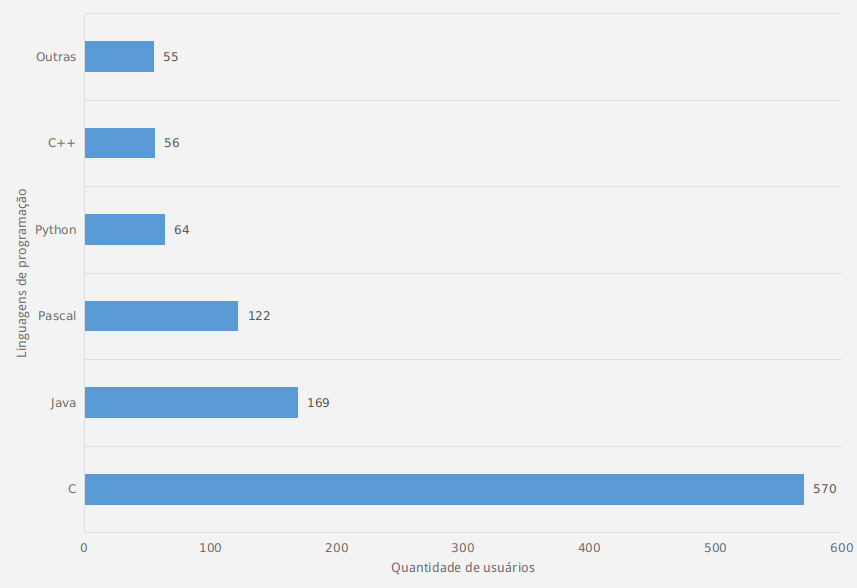
\includegraphics[scale=0.51]{images/pesquisa_linguagem_tcc.png}
  \caption{Linguagens de programação utilizadas primariamente no ensino de introdução à programação}
  \label{fig:pesquisa_linguagem_tcc}
\end{figure}

\subsection{OpenGL}
O \citeonline{OpenGL:About} é uma biblioteca gráfica para desenvolvimento de aplicações interativas. Desde sua introdução, no ano de 1992, a biblioteca OpenGL se tornou  a interface de de programação de aplicação (API) mais utilizada com suporte a 2D e 3D pela indústria. O OpenGL foi escolhido como biblioteca gráfica pela sua qualidade de ser altamente portável estando presente em várias plataformas, como Windows, Linux, Unix, MacOS, e mais. Outro motivo foi também por possuir um bom desempenho e poder ser utilizada em conjunto com várias linguagens de programação, dentre as quais foi escolhida a linguagem de programação \citeonline{C:About}.

A biblioteca gráfica \citeonline{OpenGL:About} foi escolhida em detrimento de outras por ser mais simples, porém versátil, e suas já citadas qualidades: performance, largamente utilizada, interoperável entre plataformas e por ter fácil integração com a linguagem de programação C. Outros fatores que influenciaram a sua escolha foi a vasta documentação, como websites, livros e cursos online. Alguns sites que promovem a documentação de utilização do OpenGL são o próprio site do OpenGL \url{https://opengl.org/}, o website \citeonline{LearnOpenGL:Site} e o livro OpenGL Programming Guide: The Official Guide to Learning OpenGL, Version 1.2, do autor \citeonline{Woo:1999:OPG:554539}.

A forma que o OpenGL trabalha para renderizar os objetos na tela é baseado em uma máquina de estados. Cada item renderizado pelo OpenGL fica num buffer secundário e só é renderizado quando explicitamente solicitado. Ao renderizar o buffer ele então faz a troca do buffer primário pelo secundário, exibindo assim apenas o quadro renderizado por completo, evitando assim o \textit{tearing}. \textit{Tearing} é o efeito que ocorre quando parte do frame é renderizado utilizando informações antiga, exibindo assim parte do quadro com uma imagem e outra parte com os dados novos.

\subsection{GLFW}
Segundo o site da \citeonline{GLFW:About}, GLFW é uma biblioteca gráfica de código-aberto, multi-plataforma para desenvolvimento desktop utilizando OpenGL, OpenGL ES e Vulkan. Ela é responsável por criar janelas de forma unificada entre diferentes sistemas operacionais, contextos OpenGL e receber entradas de dados e eventos.

A biblioteca GLFW foi escrita em C e possui suporte nativo para Windows, macOS e vários sistemas Unix \cite{Unix:About} que utilizam o sistema de janelas X Window System \cite{X:About}, como por exemplo Linux \cite{Linux:About} e FreeBSD \cite{FreeBSD:About}.

As motivações que levaram a escolha da biblioteca gráfica GLFW foram a criação de janelas de forma transparente entre diversos sistemas operacionais, suporte para OpenGL, suporte a vários monitores e várias janelas simultâneas, suporte para mouse, teclado e joystick, além de ser a biblioteca mais atualizada, tendo vasta documentação e grande comunidade ativa. A documentação completa da biblioteca GLFW pode ser encontrada no website da biblioteca pelo endereço \url{http://www.glfw.org/documentation.html}.

\subsection{TinyCThread}
A biblioteca \citeonline{Tinycthread:About} é uma biblioteca de código aberto escrita em C multi-plataforma capaz de criar e gerenciar threads de forma unificada e transparente em diversos sistemas operacionais. Segundo \citeonline{Tanenbaum:2007:MOS:1410217}, thread é uma forma de um processo dividir as tarefas a serem executadas de uma forma que possam ser executadas concorrentemente. Um processo que possui apenas uma thread para execução é chamado de \textit{single threading} e aplicações que possuem múltiplas threads são chamados de \textit{multi threading}. Threads podem ser executadas em paralelo, desde que o processador possua mais um núcleo, onde cada thread seria executada em um núcleo distinto.

A biblioteca TinyCThread foi escolhida pois, apesar do padrão C11 implementar suporte nativo para criação de threads da mesma forma entre diferentes sistemas operacionais, os compiladores mais antigos, e que ainda não implementam esse padrão, possuem formas distintas de criar e gerenciar as threads. Com o uso da biblioteca essa criação fica padronizada sendo possível compilar o mesmo código tanto para Linux quanto para Windows. A biblioteca também provê funcionalidades para gerenciamento de concorrência, como locks exclusivos, por exemplo o mutex, dentre outros.

\section{Atividades Desenvolvidas}
Os artefatos gerados como resultado deste trabalho são os seguintes:

\begin{itemize}
    \item A criação de uma biblioteca gráfica simplificada utilizando OpenGL e o framework GLFW
    \item A criação de uma aplicação de demonstração de utilização da biblioteca
    \item A documentação e manual de utilização
\end{itemize}

\subsection{A biblioteca gráfica}
A biblioteca gráfica descrita neste trabalho tem por intenção simplificar o uso da biblioteca OpenGL. Um dos meios utilizados para isso é a simplificação do gerenciamento da janela. Em uma aplicação OpenGL o utilizador é responsável por gerenciar tanto a janela quanto o contexto, e decidir como será realizada a renderização das formas dentro da janela. Nesta biblioteca, apesar de ainda possuir uma janela, ela é oculta e gerenciada pela própria biblioteca. Tal abordagem reduz a flexibilização oferecida pela biblioteca OpenGL, entretanto, em troca disso, obtemos uma API bastante simplificada.

Para o correto funcionamento da biblioteca é necessário criar uma janela para realizar a renderização das formas; este é o padrão de funcionamento do OpenGL. Visando a simplicidade, todo o código de criação de janelas é abstraído em uma única função. Esta função realiza várias ações, como criar a janela do OpenGL, inicializar o buffer de objetos a serem renderizados, inicializar os \textit{locks} de exclusão mútua \textit{mutex} para gerenciamento de concorrência no buffer de objetos e a inicialização da \textit{thread} que será responsável por toda a abstração de renderização do buffer de objetos na janela. Esta thread possui um laço de repetição onde é realizada a leitura do buffer de objetos contido na memória e então, renderiza os objetos de acordo com a configuração definida de cada objeto. A arquitetura proposta para a biblioteca pode ser vista na Figura ~\ref{fig:arquitetura_proposta}.

O buffer de objetos em si também não pode ser gerenciado diretamente pelo usuário. As funções expostas pela biblioteca são responsáveis por gerenciar diretamente o buffer, minimizando assim a possibilidade de erros na hora de renderizar os objetos. Cada função que desenha uma forma adiciona no buffer de objetos a configuração  correspondente ao que deve ser desenhado. Na sequência, a thread oculta faz o \textit{lock} exclusivo do buffer para que, no ato do desenho, ele não seja alterado e então, item a item, renderiza todos os objetos na janela. Após o o processo de renderização, é liberado o lock exclusivo, permitindo assim a manipulação do buffer de objetos. Este loop roda em torno de 60 vezes por segundo, podendo o número de execuções ser menor dependendo do hardware gráfico da máquina. Por se tratar de renderização de objetos muito básicos, espera-se que a média de quadros renderizados seja em torno de 60 FPS

\begin{figure}[htbp]
  \centering
  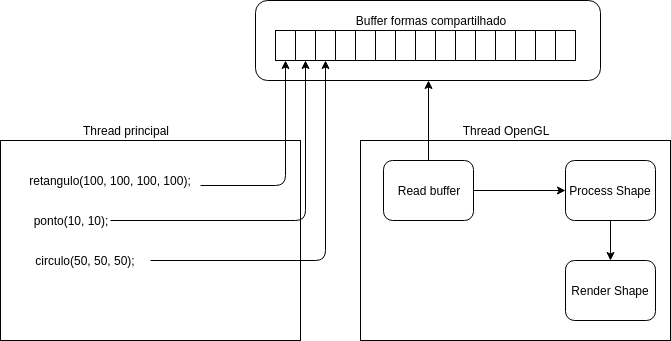
\includegraphics[scale=0.7]{images/basic_architecture.png}
  \caption{Arquitetura proposta para a biblioteca}
  \label{fig:arquitetura_proposta}
\end{figure}

A biblioteca gráfica dispõe da API abaixo:

\begin{itemize}
    \item void inicializarBiblioteca(int largura, int altura);
    \item void limparTela();
    
    \item void desfazerUltimaForma();
    \item void refazerUltimaForma();
    
    \item void definirCor(int vermelho, int verde, int azul);
    \item int* obterCor();
    
    \item void definirEspessura(int espessura);
    \item int obterEspessura();

    \item void poligono(int numeroDeVertices, GLfloat* posicoes);
    \item void ponto(int posX, int posY);
    \item void triangulo(int posX1, int posY1, int posX2, int posY2, int posX3, int posY3);
    \item void retangulo(int posX, int posY, int largura, int altura);
    \item void quadrado(int posX, int posY, int tamanhoLado);
    \item void poligonoRegular(int posX, int posY, int raio, int faces);
    \item void circulo(int posX, int posY, int raio);
    \item void pentagono(int posX, int posY, int raio);
    \item void hexagono(int posX, int posY, int raio);
    \item void decagono(int posX, int posY, int raio);
    \item void dodecagono(int posX, int posY, int raio);
    \item void linha(int posX1, int posY1, int posX2, int posY2);
    
    \item void pausar(int time);
\end{itemize}

As seções seguintes descrevem cada item da API bem como seus protótipos e o significado de cada parâmetro de entrada.

\subsubsection{Iniciando a biblioteca}
Apesar de não ter que gerenciar diretamente a janela e o laço de repetição de renderização do OpenGL manualmente, ainda se faz necessário inicializar a biblioteca manualmente, para disparar a thread secundária, responsável pela renderização dos objetos, e a criação da janela onde serão renderizadas os objetos.

A função que inicializa a biblioteca tem o seguinte protótipo:

\begin{minted}{c}
void inicializarBiblioteca(int largura, int altura);
\end{minted}

Os parâmetros de entrada são:

\begin{itemize}
    \item int largura - a largura do tamanho da janela a ser criada.
    \item int altura -  altura do tamanho da janela a ser criada.
\end{itemize}

O exemplo abaixo mostra como inicializar a biblioteca em uma aplicação C:
\begin{listing}[ht]
\begin{minted}{c}
#include <stdio.h>
#include <graphics.h>

int main() {
    inicializarBiblioteca(800, 600);

    retangulo(0, 0, 200, 100);
    limparTela();

    getchar();
    return 0;
}
\end{minted}
\caption{Inicializando a biblioteca}
\label{lst:inicializando_biblioteca}
\end{listing}

\begin{figure}[!htbp]
  \centering
  \includegraphics[scale=0.7]{images/exemplo_initWindow.JPG}
  \caption{Exemplo inicialização da biblioteca}
  \label{fig:exemplo_initWindow}
\end{figure}

\subsubsection{Limpando a tela}
A biblioteca descrita neste trabalho permite que a janela seja limpa, removendo assim todas os objetos renderizados e reiniciando a janela para seu estado inicial.

A função que limpa a janela já foi utilizada anteriormente e pode ser encontrada no exemplo ~\ref{lst:inicializando_biblioteca}

\subsubsection{Desfazer último desenho}
Em uma aplicação, é comum se arrepender de sua última ação e portanto, querer desfazê-la. A biblioteca aqui implementada possui uma função específica para esta ação. Ela pode ser utilizada múltiplas vezes e a cada vez um objeto é removido da tela.

A função que desfaz o último desenho tem o seguinte protótipo:

\begin{minted}{c}
void desfazerUltimaForma();
\end{minted}

\subsubsection{Refazer o último desenho}
Refazer o último desenho é uma opção da mesma forma que desfazer o último desenho, você pode se arrepender e desfazer a opção de desfazer. A cada vez que a função for chamada, um desenho será restaurado. A ordem de restauração é baseada na estrutura de dados pilha, portanto o último objeto removido será o primeiro objeto restaurado. Essa função só pode ser executa caso invocada imediatamente após a função de desfazer, pois caso seja inserida um novo objeto após ter desfeito o último desenho, a pilha de ações será descartada.

A função que refaz o último desenho tem o seguinte protótipo:

\begin{minted}{c}
void refazerUltimaForma();
\end{minted}

\subsubsection{Alterado a cor de preenchimento de um objeto} \label{api_definirCor}
A grande maioria, senão todas, as biblioteca citadas nos trabalhos correlatos permitem a definição de uma cor de preenchimento para o objeto a ser desenhado.

A função que permite alterar a cor de um objeto tem o seguinte protótipo:

\begin{minted}{c}
void definirCor(int vermelho, int verde, int azul);
\end{minted}

Os parâmetros de entrada são:

\begin{itemize}
    \item int vermelho - um inteiro de 0 a 255 representando a tonalidade de vermelho do padrão RGB.
    \item int verde - um inteiro de 0 a 255 representando a tonalidade de verde do padrão RGB.
    \item int azul - um inteiro de 0 a 255 representando a tonalidade de azul do padrão RGB.
\end{itemize}

\subsubsection{Obter a cor de preenchimento do objeto}
Assim como podemos definir a cor de preenchimento de um objeto, também é possível obtermos a cor de preenchimento atual. Esta função se faz útil quando, por exemplo, queremos criar um objeto de uma nova cor mas queremos manter a cor antiga, porém não é conhecido a cor de preenchimento atual. Assim como visto em \ref{api_definirCor}, como a função \textit{definirCor} recebe 3 argumentos de entrada, a saída é um ponteiro representando um array de inteiros de tamanho 3, representando as cores RGB.

A função que obtém a cor atual de uma forma tem o seguinte protótipo:

\begin{minted}{c}
int* obterCor();
\end{minted}

A saída do método é um ponteiro para um array contendo 3 posições e seus valores são descritos conforme a lista abaixo:

\begin{itemize}
    \item int cor[0] - um inteiro de 0 a 255 representando a tonalidade de vermelho do padrão RGB.
    \item int cor[1] - um inteiro de 0 a 255 representando a tonalidade de verde do padrão RGB.
    \item int cor[2] - um inteiro de 0 a 255 representando a tonalidade de azul do padrão RGB.
\end{itemize}

O exemplo abaixo mostra como obter a cor atual de uma forma em uma aplicação C:

\begin{minted}{c}
#include <stdio.h>
#include <graphics.h>

int main() {
    inicializarBiblioteca(800, 600);

    definirCor(255, 0, 127);
    retangulo(0, 0, 200, 100);

    int* corAtual = obterCor();

    getchar();
    return 0;
}
\end{minted}

\subsubsection{Definindo o tamanho de um objeto}
Alguns objetos podem ter seu tamanho alterado. Para que tenha efeito, a função \textit{definirTamanho} deve ser invocada anteriormente a uma função de desenho de forma. Após chamado o método, todos os objetos desenhados após a chamada serão desenhados com o novo tamanho definido. Atualmente apenas o objeto \textit{ponto} pode ter seu tamanho alterado.

A função que define o tamanho de uma forma tem o seguinte protótipo:

\begin{minted}{c}
void definirTamanho(int tamanho);
\end{minted}

O exemplo abaixo mostra como definir o tamanho de uma forma em uma aplicação C:

\begin{minted}{c}
#include <stdio.h>
#include <graphics.h>

int main() {
    inicializarBiblioteca(800, 600);

    definirTamanho(50);
    ponto(100, 100);

    getchar();
    return 0;
}
\end{minted}

\subsubsection{Obtendo o tamanho de um objeto}
Da mesma forma que é possível definir o tamanho de um objeto, esta função permite obter o valor atual do tamanho de desenho de objetos. Esta função é útil quando você quer desenhar um objeto em novo tamanho e deseja retornar o tamanho anterior para os próximos objetos, porém você não possui o conhecimento de qual o valor atual do tamanho da forma.

A função que como obter o tamanho atual de uma forma tem o seguinte protótipo:

\begin{minted}{c}
int obterTamanho();
\end{minted}

O exemplo abaixo mostra como obter o tamanho atual de uma forma em uma aplicação C:

\begin{minted}{c}
#include <stdio.h>
#include <graphics.h>

int main() {
    inicializarBiblioteca(800, 600);

    definirTamanho(50);
    ponto(100, 100);

    int tamanhoAtual = obterTamanho();

    getchar();
    return 0;
}
\end{minted}

\subsubsection{Desenhando um polígono}
Um polígono é uma figura geométrica composta por 3 ou mais vértices. Um polígono pode ser desenhado de forma livre e a função que desenha um polígono tem o seguinte protótipo:

\begin{minted}{c}
void poligono(int numeroDeVertices, GLfloat* posicoes);
\end{minted}

Os parâmetros de entrada são:

\begin{itemize}
    \item int numeroDeVertices - número de vértices que o seu polígono possui
    \item GLfloat* posicoes - um array contendo as posições de cada vértice. O array deve possuir um tamanho par definido pela fórmula \(tamanho = 2 \times numeroDeVertices \), pois as posições pares representam as posições X dos vértices e as posições ímpares representam as posições Y, par a par. Os pares devem ser definidos sequencialmente. Para desenhar um triângulo, seria então necessário um array de 6 posições. Utilizando um triângulo como exemplo, vamos utilizar os pontos (0, 0), (200, 0) e (100, 200). O array de posições então seria \textit{GLfloat posicoes[6] = \{0, 0, 200, 0, 100, 200\};}.
\end{itemize}

O exemplo abaixo mostra como desenhas um polígono em uma aplicação C:

\begin{minted}{c}
#include <stdio.h>
#include <stdlib.h>
#include <graphics.h>

int main() {
    inicializarBiblioteca(800, 600);

    GLfloat posicoes[] = {
        320, 100,
        400, 300,
        800, 50,
        520, 10,
        340, 40
    };
    poligono(5, posicoes);

    getchar();
    return 0;
}
\end{minted}

\subsubsection{Desenhando um ponto}
A função que desenha um ponto tem o seguinte protótipo:

\begin{minted}{c}
void ponto(int posX, int posY);
\end{minted}

Os parâmetros de entrada são:

\begin{itemize}
    \item int posX - a posição X do ponto.
    \item int posY - a posição Y do ponto.
\end{itemize}

\subsubsection{Desenhando um triângulo}
Triângulos são uma das formas mais básicas e utilizadas, pois todos os polígonos convexos pode ser decompostos em vários triângulos. A função que desenha um triângulo tem o seguinte protótipo:

\begin{minted}{c}
void triangulo(
    int posX1, int posY1,
    int posX2, int posY2,
    int posX3, int posY3
);
\end{minted}

Os parâmetros de entrada são:

\begin{itemize}
    \item int posX1 - a posição X da vértice 1 do triângulo.
    \item int posY1 - a posição Y da vértice 1 do triângulo.

    \item int posX2 - a posição X da vértice 2 do triângulo.
    \item int posY2 - a posição Y da vértice 2 do triângulo.

    \item int posX3 - a posição X da vértice 3 do triângulo.
    \item int posY3 - a posição Y da vértice 3 do triângulo.
\end{itemize}

\subsubsection{Desenhando um retângulo}
Retângulos são formas geométricas que possuem 4 ângulos retos e também são bastante utilizados para desenhos além de ser uma das formas mais básicas. A função que desenha um retângulo tem o seguinte protótipo:

\begin{minted}{c}
void retangulo(int posX, int posY, int largura, int altura);
\end{minted}

Os parâmetros de entrada são:

\begin{itemize}
    \item int posX - posição X do retângulo. Representa o vértice inferior esquerdo do retângulo.
    \item int posY - posição y do retângulo. Representa o vértice inferior esquerdo do retângulo.
    \item int altura - altura do triângulo.
    \item int largura - largura do triângulo.
\end{itemize}

\subsubsection{Desenhando um quadrado}
Um quadrado é um polígono considerado especial, pois trata-se de um retângulo que possui largura e altura de mesmo tamanho.

A função que desenha um quadrado tem o seguinte protótipo:

\begin{minted}{c}
void quadrado(int posX, int posY, int tamanhoLado);
\end{minted}

Os parâmetros de entrada são:

\begin{itemize}
    \item int posX - posição X do quadrado. Representa o vértice inferior esquerdo do quadrado.
    \item int posY - posição Y do quadrado. Representa o vértice inferior esquerdo do quadrado.
    \item int tamanhoLado - tamanho do lado do quadrado.
\end{itemize}

\subsubsection{Desenhando um polígono regular}
Um polígono regular é um polígono convexo com \textit{n} faces onde cada face possui o mesmo tamanho e todos os ângulos internos são iguais. Alguns exemplos de polígonos regulares são triângulos retângulos, quadrados, pentagonos, dodecagonos, etc.

Segundo \citeonline{PoligonoConvexos:BrasilEscola}, ``um polígono é convexo quando todos os pontos de um segmento de reta que possui as extremidades no interior do polígono também estão dentro dele. Sendo assim, se for possível encontrar pelo menos um segmento de reta que possui as extremidades dentro do polígono e, ao mesmo tempo, um ponto fora dele, esse polígono não será convexo''.

A função que desenha um polígono regular tem o seguinte protótipo:

\begin{minted}{c}
void poligonoRegular(int posX, int posY, int raio, int faces);
\end{minted}

Os parâmetros de entrada são:

\begin{itemize}
    \item int posX - posição X onde do polígono regular. Representa o centro de onde será desenhado o objeto.
    \item int posY - posição Y onde do polígono regular. Representa o centro de onde será desenhado o objeto.
    \item int raio - tamanho do raio que do polígono regular.
    \item int faces - o número de faces que do polígono regular.
\end{itemize}

O exemplo abaixo mostra como desenhar um polígono regular azul em uma aplicação C:

\begin{minted}{c}
#include <stdio.h>
#include <stdlib.h>
#include <graphics.h>

int main() {
    inicializarBiblioteca(800, 600);

    definirCor(0, 0, 255);
    poligonoRegular(300, 300, 100, 7);

    getchar();
    return 0;
}
\end{minted}

\subsubsection{Desenhando um círculo}
O círculo é uma forma geométrica que possui virtualmente infinitos vértices.

A função que desenha um círculo tem o seguinte protótipo:

\begin{minted}{c}
void circulo(int posX, int posY, int raio);
\end{minted}

Os parâmetros de entrada são:

\begin{itemize}
    \item int posX - posição X do centro do círculo.
    \item int posY - posição Y do centro do círculo.
    \item int raio - raio do círculo.
\end{itemize}

\subsubsection{Desenhando um pentágono}
Um pentágono é um polígono regular composto por 5 vértices.

A função que desenha um pentágono tem o seguinte protótipo:

\begin{minted}{c}
void pentagono(int posX, int posY, int raio);
\end{minted}

Os parâmetros de entrada são:

\begin{itemize}
    \item int posX - posição X do centro do pentágono.
    \item int posY - posição Y do centro do pentágono.
    \item int raio - raio do pentágono.
\end{itemize}

\subsubsection{Desenhando uma linha}
Dado 2 pontos A e B, uma linha é um segmento de reta que liga os pontos A e B.

A função que desenha uma linha tem o seguinte protótipo:

\begin{minted}{c}
void linha(int posX1, int posY1, int posX2, int posY2);
\end{minted}

Os parâmetros de entrada são:

\begin{itemize}
    \item int posX1 - posição do X1 da linha.
    \item int posY1 - posição do Y1 da linha.
    \item int posX2 - posição do X2 da linha.
    \item int posY2 - posição do Y2 da linha.
\end{itemize}

O exemplo abaixo mostra como desenhar uma linha que corta a janela de desenho verticalmente em uma aplicação C:

\begin{minted}{c}
#include <stdio.h>
#include <graphics.h>

int main() {
    inicializarBiblioteca(1366, 768);

    linha(
        0, 0,
        1366, 768
    );

    getchar();
    return 0;
}
\end{minted}

\section{Estado Atual do Desenvolvimento}
[TODO] \textbf{Falar que tudo o que era previsto foi feito}

\section{Trabalhos Futuros}
[TODO] \textbf{Pensar em algumas features e melhorias}

\begin{itemize}
    \item Suporte multi janelas
    \item controle de janela opcional
    \item edição da forma já adicionada no buffer
    \item suporte 3D
\end{itemize}

\chapter{Considerações Finais}
[TODO] \textbf{Não faço a menor ideia do que escrever aqui ainda}

\section{Dificuldades Encontradas}

\begin{itemize}
  
  \item Compilar multi plataforma
  \item Instalação da biblioteca GLFW
  \item Corrupção da memória HEAP no Windows
  \item Instalação da biblioteca no Code::Blocks
  
\end{itemize}

\section{Conclusão}
[TODO] \textbf{Concluir!}

%\chapter{Desenvolvimento}
%Um ou mais capítulos (por exemplo um para testes)

% ---
% Conclusão
% ---
\iffalse
\chapter*[Conclusão]{Conclusão}
\addcontentsline{toc}{chapter}{Conclusão}
%TCC:
Descrever aqui as conclusões e/ou considerações finais.
Destacar as contribuições originais do trabalho.
Propor trabalhos futuros em continuidade ao trabalho realizado.
\fi

% ----------------------------------------------------------
% ELEMENTOS PÓS-TEXTUAIS
% ----------------------------------------------------------
\postextual

%\nocite{babel}
% ----------------------------------------------------------
% Referências bibliográficas
% ----------------------------------------------------------
\bibliography{referencias}


%% ----------------------------------------------------------
%% Apêndices TCC: só mantenha se for pertinente.
%% ----------------------------------------------------------

\iffalse
% ---
% Inicia os apêndices
% ---
\begin{apendicesenv}

% Imprime uma página indicando o início dos apêndices
\partapendices
% ----------------------------------------------------------
\chapter{Quisque libero justo}
% ----------------------------------------------------------

\lipsum[50]

% ----------------------------------------------------------
\chapter{Coisas que fiz e que achei interessante mas não tanto para entrar no corpo do texto}
% ----------------------------------------------------------
\lipsum[55-57]
\end{apendicesenv}
\fi
% ---


% ----------------------------------------------------------
% Anexos %TCC: so mantenha se pertinente.
% ----------------------------------------------------------

\iffalse
% ---
% Inicia os anexos
% ---
\begin{anexosenv}

% Imprime uma página indicando o início dos anexos
\partanexos
% ---
\chapter{Eu sempre quis aprender latim}
% ---
\lipsum[30]

% ---
\chapter{Coisas que eu não fiz mas que achei interessante o suficiente para colocar aqui}
% ---

\lipsum[31]

% ---
\chapter{Fusce facilisis lacinia dui}
% ---

\lipsum[32]
\end{anexosenv}
\fi

%---------------------------------------------------------------------
% INDICE REMISSIVO
%---------------------------------------------------------------------

\printindex



\end{document}
